\documentclass{article}

% Language setting
% Replace `english' with e.g. `spanish' to change the document language
\usepackage[english]{babel}

% Set page size and margins
% Replace `letterpaper' with `a4paper' for UK/EU standard size
\usepackage[letterpaper,top=2cm,bottom=2cm,left=3cm,right=3cm,marginparwidth=1.75cm]{geometry}

% Useful packages
\usepackage{amsmath}
\usepackage{amssymb}
\usepackage{graphicx}
\usepackage{inconsolata}
\usepackage{minted}
\usepackage[colorlinks=true, allcolors=blue]{hyperref}

\title{Innlevering 1: Del 2-5}
\author{Skrevet av André Hansen}

\begin{document}
\maketitle

\begin{abstract}
Dette er det løsning for første innlevering som dekker del 2-5 i pensum. Jeg kommer til å behandle denne innleverigen på lik linje som selve eksamenen.
\end{abstract}

\section{Uten hjelpemidler}

\subsection{Oppgave 1: Betrakt rekka 5+9+13+17+21+...}

\subsubsection{Hva er det tolvte leddet i denne rekka?}

Først defineres en eksplisitt formel med den eksplisitte formelen for aritmetiske rekker

\begin{align*}
    a_n &= k(n-1)+a_1 \\
    a_1 &= 5 \\
    k &= a_2 - a_1 = 4 \\
    a_n &= 4(n-1)+5
\end{align*}

så brukes resultatet for å regne $a_{12}$

\begin{align*}
    a_{12} &= 4(12-1)+5 = 49
\end{align*}

\subsubsection{Hva er summen av de tolv første leddene}

Først og fremst defineres en eksplisitt formel med å bruke $\Sigma$ for å regne $s_n$

\begin{align*}
    s_n &= \sum_{i=1}^{n} 4(i-1)+5 \\
    &= \sum_{i=1}^{n} 4i + 1 \\
    &= 4 \sum_{i=1}^{n} i + \sum_{i=1}^{n} 1 \\
    &= 4 \frac{n(n+1)}{2} + n \\
    &= 4 \frac{n^2+n}{2} + n \\
    &= 2n^2 + 3n
\end{align*}

Derreter regnes $n_{12}$ eksplisitt

\begin{align*}
    s_{12} &= 2 \cdot 12^2 + 3 \cdot 12 \\
    &= 2 \cdot 144 + 36 \\
    &= 324
\end{align*}

\subsubsection{Hva er summen av de n første leddene i denne rekka}

Summen for de n første leddene ble definert i oppgaven over. Men den er: $2n^2 + 3n$

\subsection{Oppgave 2: Betrakt rekka $\frac{15}{16} + \frac{3}{4} + \frac{3}{5} + \frac{12}{25}$}

\subsubsection{Begrunn hvorfor rekka er geometrisk og hvorfor den konvergerer}

Rekka er geometrisk fordi den kan defineres med $a_{n+1}=a_n k + a_1$

variabelen $k$ avgjør om rekka konvergerer og i denne rekka er $k=0.8$ som betyr at den konvergerer.

En rekke konvergerer når $k \in [0, 1]$

\subsubsection{Funn summen av rekka}

Summen for en kovergerende geometrisk rekker er $\frac{a_1}{1-k}$

Dermed:

\begin{align*}
    & \frac{\frac{15}{16}}{1-\frac{8}{10}} \\
    &= \frac{\frac{15}{16}}{\frac{2}{10}} \\ 
    &= \frac{15}{16} \div \frac{2}{10} \\
    &= \frac{15}{16} \cdot \frac{10}{2} \\
    &= \frac{150}{32} \\
    &= \frac{75}{16}
\end{align*}

Summen er dermed: $\frac{75}{16}$

\subsection{Oppgave 3: Bruk fortegnsskjema til å finne konvergeringsområdet til rekka: $1+\frac{3+x}{2x}+(\frac{3+x}{2x})^2+(\frac{3+x}{2x})^3+...$}


Dette kan defineres som en gemoetisk rekke med k:
\[
k = \frac{3+x}{2x}
\]

Dermed har vi ulikheten
\[
\left|\frac{3+x}{2x}\right| < 1 \;\Longleftrightarrow\; (x+3)^2 < (2x)^2 \\
x^2+6x+9 < 4x^2 \;\Longleftrightarrow\; 0 < 3x^2 - 6x - 9 \;\Longleftrightarrow\; 0 < (x-3)(x+1)
\]

Dermed kan et fortegnsskjema for $(x-3)(x+1)$ lages
\[
x \in (-\infty,-1)\cup(3,\infty), \quad x\neq 0.
\]

konvergeringsområdet blir da:
\[
(-\infty,-1)\cup(3,\infty).
\]

\subsection{Oppgave 4: Regn ut integralene}

\subsubsection{$\int_{0}^{1} (e^{4x}+2x) dx$}

\begin{align*}
    & \int_{0}^{1} (e^{4x}+2x) dx \\
    & = [\frac{1}{4} e^{4x} + x^2]^1_0 \\
    &= \frac{1}{4} e^4 + 1^2 - \frac{1}{4}1 \\
    &= \frac{1}{4} e^4 + \frac{3}{4}
\end{align*}

\subsubsection{$\int_{0}^{3} (x^2-2x-1)^3(2x-2) dx$}

Denne løsningen bruker rå makt

\begin{align*}
    & \int_{0}^{3} (x^2-2x-1)^3(2x-2) dx \\
    &= \int_{0}^{3} (x^2-2x-1)^2(x^2-2x-1)(2x-2) dx \\
    &= \int_{0}^{3} (x^4-4x^2+2x^2+4x+1)(x^2-2x-1)(2x-2) dx \\
    &= \int_{0}^{3} (x^6-6x^5+9x^4+4x^3-7x^2-8x-1)(2x-2) dx \\
    &= \int_{0}^{3} 2x^7-12x^6+18x^5+8x^4-14x^3-16x^2-2x dx \\
    &= [\frac{2}{8}x^8-\frac{14}{7}x^7+\frac{30}{6}x^6-\frac{10}{5}x^5-\frac{22}{4}x^4-\frac{2}{3}x^2+7x^2+2x]^3_0 \\
    &= [\frac{1}{4}x^8-2x^7+5x^6-2x^5-\frac{11}{2}x^4-\frac{2}{3}x^3+7x^2+2x]^3_0 \\
    &= (\frac{1}{4}*3^8-2*3^7+5*3^6-2*3^5-\frac{11}{2}*3^4-\frac{2}{3}*3^3+7*3^2+2*3) \\
    &- (\frac{1}{4}*1^8-2*1^7+5*1^6-2*1^5-\frac{11}{2}*1^4-\frac{2}{3}*1^3+7*1^2+2*1) \\
    &= (\frac{1}{4}*3^8-2*3^7+5*3^6-2*3^5-\frac{11}{2}*3^4-\frac{2}{3}*3^3+7*3^2+2*3) - \frac{49}{12} \\
    &= (\frac{1}{4}*6561- 2*2187+5*729-2*243-\frac{11}{2}*81-\frac{2}{3}*27+7*9+6) - \frac{49}{12} \\
    &= (\frac{6561}{4}- 2*2187+5*729-2*243-\frac{891}{2}-\frac{54}{3}+63+6) - \frac{49}{12} \\
    &= (\frac{6561}{4}- 4374+3645-486-\frac{891}{2}-\frac{54}{3}+63+6) - \frac{49}{12} \\
    &= \frac{80}{3}
\end{align*}

\subsubsection{$\int e^{2x}(x^2+3x+1) dx$}

Denne løsningen bruker delvis integrasjon

\begin{align*}
    & \int e^{2x}(x^2+3x+1) dx \\ 
    &= \frac{1}{2} e^{2x} (x^2+3x+1) - \int \frac{1}{2} e^{2x} (2x+3) \\
    &= \frac{1}{2} e^{2x} (x^2+3x+1) - \frac{1}{2} \int e^{2x} (2x+3) \\
    &= \frac{1}{2} e^{2x} (x^2+3x+1) - \frac{1}{2} ( \frac{1}{2} e^{2x} (2x+3) - \int \frac{1}{2} e^{2x}2) \\
    &= \frac{1}{2} e^{2x} (x^2+3x+1) - \frac{1}{2} ( \frac{1}{2} e^{2x} (2x+3) - \frac{1}{2} e^{2x}) \\
    &= \frac{1}{2} e^{2x} (x^2+3x+1) - \frac{1}{2} * \frac{1}{2} e^{2x} ((2x+3) - 1) \\
    &= \frac{1}{2} e^{2x} ((x^2+3x+1) - \frac{1}{2} ((2x+3) - 1)) \\
    &= \frac{1}{2} e^{2x} ((x^2+3x+1) - \frac{2x+2}{2}) \\
    &= \frac{1}{2} e^{2x} ((x^2+3x+1) - (x-1)) \\
    &= \frac{1}{2} e^{2x} ((x^2+2x+2)) \\ 
    &= e^{2x} (\frac{1}{2} x^2 + x) + C
\end{align*}

\subsubsection{$\int \frac{3x-37}{x^2-3x-4}$}

her brukes brøkssplitting

\begin{align*}
    & \frac{3x-37}{x^2-3x-4} \\
    &= \frac{A}{x+1} + \frac{B}{x-4} \\
    &= \frac{A(x-4)}{(x+1)(x-4)} + \frac{B(x+1)}{(x+1)(x-4)} \\
    &= A(x-4) + B(x+1) = 3x - 37 \\
    & x=4 \rightarrow B(5) = 15 - 37 \\
    & B = \frac{-22}{5} \\
    & x = -1 \rightarrow -5A = -15 -37 \\
    &= A = \frac{52}{5}
\end{align*}

Nå som $A$ og $B$ er definert kan vi regne ut integralene

\begin{align*}
    & \int \frac{\frac{52}{5}}{\frac{(x-1)}{1}} dx + \int \frac{\frac{-22}{5}}{\frac{(x-4)}{1}} \\
    &= \int \frac{52}{5} \div \frac{(x+1)}{1} + \int \frac{-22}{5} \div \frac{x-4}{1} \\
    &= \int \frac{52}{5(x+1)} + \int \frac{-22}{5(x-4)} \\
    &= \frac{52}{5} \int \frac{1}{(x+1)} + \frac{-22}{5} \int \frac{1}{(x-4)} \\
    &= \frac{52}{5} (ln|x| + x) - \frac{22}{5} (ln|x| - \frac{1}{4}{x}) \\
    &= \frac{52(ln|x| + x)}{5}  - \frac{22(ln|x| - \frac{1}{4}{x})}{5} \\
    &= \frac{52(ln|x| + x) - 22(ln|x| - \frac{1}{4}{x})}{5} \\
    &= \frac{52ln|x| + 52x - 22ln|x| - \frac{-22}{4}{x}}{5} \\
    &= \frac{30ln|x| + \frac{230}{4}x}{5} \\
    &= \frac{30ln|x| + \frac{115}{2}x}{5} \\
    &= 6ln|x| + \frac{575}{2}x+C
\end{align*}

\subsubsection{$\int 8xe^{2x^2}dx$}

\begin{align*}
    & \int 8xe^{2x^2}dx \\
    &= \int 8xe^{u} \frac{du}{4x} \\
    &= 2 \int e^{u} \\ 
    &= 2e^{2x^2} + C
\end{align*}

\subsection{Oppgave 5: La $f(x)=5x^2+3, D_f=[-1, 2]$ Hva er volumet av omdreiningslegemet som framkommer ved å dreie grafen til $f 360^\circ$ om x-aksen?}

For å finne omdreiningslegemet må integralet $\pi \int_{-1}^{2} (5x^2+3)^2$ løses

\begin{align*}
    V &= \pi \int_{-1}^{2} (5x^2+3)^2 \\
    &= \pi \int_{-1}^{2} 25x^4 + 30x^2 + 9 \\
    &= \pi [\frac{25}{5} x^5 + \frac{30}{3} x^3 + 9x]^2_{-1} \\
    &= \pi [5x^5 + 10 x^3 + 9x]^2_{-1} \\
    &= \pi ((5 * 2^5 + 10*2^3 + 9*2) - (5(-1)^2 + 10(-1)^3 + 9(-1))) \\
    &= \pi ((160 + 80 + 18) - (-5-10-9)) \\
    &= \pi (258 + 25) \\ 
    &= \pi (258 + 25) \\
    &= \pi 283
\end{align*}

\subsection{Oppgave 6: Regn ut itegral}

funksjonen er 3(x+1)(x-2) fordi den krysser -1 og 2 i x aksen.

For å finne arealet av det avgrenset området regnes det i tre separate integraler:

\begin{align*}
    &= \int_{-3}^{-1}3(x+1)(x-2)dx  + \int_{-1}^{2}3(x+1)(x-2)dx + \int_{2}^{3}3(x+1)(x-2)dx \\
    &= 3 (\int_{-3}^{-1}(x+1)(x-2)dx  + \int_{-1}^{2}(x+1)(x-2)dx + \int_{2}^{3}(x+1)(x-2)dx) \\
    &= 3 (\int_{-3}^{-1}(x^2-x-2) dx  + \int_{-1}^{2}(x^2-x-2) dx + \int_{2}^{3}(x^2-x-2) dx) \\
    &= 3 (\int_{-3}^{-1}(x^2-x-2) dx  + \int_{-1}^{2}(x^2-x-2) dx + \int_{2}^{3}(x^2-x-2) dx) \\
    &= 3 ([\frac{1}{3}x^3 - \frac{1}{2} x^2 - 2x]^{-1}_{-3} + [\frac{1}{3}x^3 - \frac{1}{2} x^2 - 2x]^2_{-1} + [\frac{1}{3}x^3 - \frac{1}{2} x^2 - 2x]^3_2) \\
    &= 3 (((\frac{1}{3}(-1)^3 - \frac{1}{2} (-1)^2 - 2(-1)) - (\frac{1}{3}(-3)^3 - \frac{1}{2} (-3)^2 - 2(-3))) \\
    &+ ((\frac{1}{3}(2)^3 - \frac{1}{2} (2)^2 - 2(2)) - (\frac{1}{3}(-1)^3 - \frac{1}{2} (-1)^2 - 2(-1))) \\
    &+ ((\frac{1}{3}(3)^3 - \frac{1}{2} (3)^2 - 2(3)) - (\frac{1}{3}(2)^3) - \frac{1}{2} (2)^2 - 2(2))) \\
    &= 3 (((\frac{-1}{3}-\frac{1}{2}+2) - (\frac{-27}{3}-\frac{9}{2}+6)) \\
    &+ ((\frac{8}{3}-\frac{4}{2}-4) - (\frac{-1}{3})-\frac{1}{2}+2) \\
    &+ ((\frac{27}{3} - \frac{9}{2} - 6) - (\frac{8}{3}-\frac{4}{2}-4))) \\
    &= 3 (((\frac{-2}{6}-\frac{3}{6}+\frac{12}{6}) - (\frac{-54}{6}-\frac{27}{6}+\frac{36}{6})) \\
    &+ ((\frac{16}{6}-\frac{12}{6}-\frac{24}{6}) - (\frac{-2}{6})-\frac{3}{6}+\frac{12}{6}) \\
    &+ ((\frac{54}{6} - \frac{27}{6} - \frac{36}{6}) - (\frac{16}{6}-\frac{12}{6}-\frac{24}{6}))) \\
    &= 3 (((\frac{12-2-3}{6}) - (\frac{36-27-54}{6})) \\
    &+ ((\frac{16-12-24}{6}) - (\frac{12-3-2}{6})) \\
    &+ ((\frac{54-27-36}{6}) - (\frac{16-12-24}{6}))) \\
    &= 3 ((\frac{7}{6} - \frac{-45}{6}) + (\frac{-20}{6} - \frac{7}{6}) + (\frac{-9}{6} - \frac{-20}{6})) \\ 
    &= 3 (\frac{52}{6} + \frac{-27}{6} + \frac{11}{6}) \\
    &= 3 (\frac{52-27+11}{6}) \\
    &= 3 (\frac{36}{6}) \\
    &= 18
\end{align*}

\section{Med hjelpemidler}

\subsection{Oppgave 7: Bevis ved induksjon at $4+9+14+19+...+(5n-1)=\frac{n}{2}(5n+3)$}

starten på beviser består av å sjekke om $P(1)$ stemmer

$$P(1) : 4 = \frac{1}{2}(5+3) \rightarrow 4 = 4$$

$P(1)$ stemmer

Jeg antar at utsagnet er sant for alle naturlige tall $n = k \in \mathbb{N}$

$4+9+14+19+...+(5k-1)=\frac{k}{2}(5k+3)$

For å bevise dette må utsagnet $n = k + 1$ også være sant:

\begin{align*}
    4+9+14+19+...+(5k-1)+(5(k+1)-1) &= \frac{k+1}{2}(5(k+1)+3) \\
    4+9+14+19+...+(5k-1)+(5(k+1)-1) &= \frac{k}{2}(5k+3) + (5(k+1)-1) \\
    &= \frac{k+1}{2}(5(k+1)+3)
\end{align*}

$P(n)$ stemmer og er bevist med induksjon

\textbf{Q.E.D}

\subsection{Oppgave 8: Kontrapositivt bevis}

Har ikke lært nokk til å gjøre denne oppgaven :(

\subsection{Oppgave 9: Trekanttallene er tallfølgen gitt ved $T_n = [\frac{1}{2} n(n+1)]^{\infty}_{n=1}$}

\subsubsection{Med utrykket for $T_n$ som utganspunkt, skriv et program som skriver ut summen av de 1, 2, 3, ... ,10 første trekanttallene}

Det kan regnes ut med Python:

\begin{verbatim}
# definerer t(n)
t = lambda n: 1/2 * n * (n+1)

# altid et heltall
def T(n) -> int:
    s = []
    for i in range(n+1):
        s.append(t(i))
    return sum(s)

# printer summen fra 1 til 10
for n in range(1, 11):
    print(f"T({n}) : {T(n)}")
\end{verbatim}

Resultat av å kjøre koden:

\begin{verbatim}
T(1) : 1.0
T(2) : 4.0
T(3) : 10.0
T(4) : 20.0
T(5) : 35.0
T(6) : 56.0
T(7) : 84.0
T(8) : 120.0
T(9) : 165.0
T(10) : 220.0
\end{verbatim}

\subsubsection{Hva er den tiende sentrerte femkanttallet $SF_{10}$}

$SF_{10}$ kan regnes med programmet:

\begin{verbatim}
    n = 10
    s = 1

    for i in range(1, n+1):
        s += 5*i -5

    print(s)
\end{verbatim}

$SF_{10} = 226$

\subsubsection{Hva er den eksplisitte formelen for $SF_n$}

$SF_n$ kan defineres på lukket form:  $1 + \sum_{i=1}^{n} 5(i)-5$

Dermed kan notasjonen konverteres til et eksplisitt uttrykk

\begin{align*}
    SF_n &= 1 +\sum_{i=1}^{n} 5(i)-5 \\ 
    &=  1 +5 \sum_{i=1}^{n} i-1 \\ 
    &=  1 +5 ( \sum_{i=1}^{n} i - \sum_{i=1}^{n} 1 ) \\
    &=  1 +5 ( \frac{n(n+1)}{2} - {n} ) \\
    &=  1 +5 ( \frac{n^2-n}{2} ) \\
    &=  1 +\frac{5}{2} n^2- \frac{5}{2}n
\end{align*}

\subsection{Oppgave 10: For å komme i form til å løpe mila under arrangementet Midnight Sun Marathon, ønsker Atle å løpe stadig lengre distanser. Han tenker å løpe 2,6 km første gang, og derreter øke distansen med 0,2 km hver gang. Han setter som mål å ha løpt til sammen 260km før arrangementet}

\subsubsection{Bruk en aritmetisk rekke til å finne ut hvor mange ganger Atle må løpe for å nå målet}

Den totale distansen Atle har løpt kan skrives som : $\sum^n_{i=1} 2.6+(0.2(i-1))$

For å finne hvor mange ganger Atle må løpe for å nå målet kan ligningen: $\sum^n_{i=1} 2.6+(0.2(i-1))=260$ løses med CAS

$\sum^n_{i=1} 2.6+(0.2(i-1))=260 \rightarrow n = 40$

Han må løpe 40 ganger for å nå målet

\subsubsection{Argumenter for at hvis Atle når målet, er han i stand til å løpe mila under Midnight Sun Marathon}

På Atle sin 40'ende og siste løpetur løper han 10,4km som er mer en det han skal løpe under Midnight Sun Marathon

\subsection{Opgpave 11: Det viser seg at t år etter planting vokser en bestemt type eukalyptustre med en hastighet gitt ved $f(t)=0.2+\frac{2}{(t+2)^2}$}

\subsubsection{Hvor mye vokser et eukalyptustre i løpet av det andre året etter det ble plantet?}

Formelen for hastighet er gitt ved :  $f(t)=0.2+\frac{2}{(t+2)^3}$

Dermed kan lengden planetn har vokst regnes ut med : $\int_{1}^{2}f(t)$ i CAS

$\int_{1}^{2}0.2+\frac{2}{(t+2)^3}=0.249$

\subsubsection{Hvor lang tid tar det fra et eukalyptustre blir plantet til det har vokst 2,25m}

Legnden til treet kan defineres ved $\int f(t)$

\begin{align*}
    F(t) &= \int f(t) \\
    &= \int 0.2+\frac{2}{(t+2)^3} \\
    &= \frac{1}{5}t - \frac{2}{2(t+2)^2}
\end{align*}

For å finne tiden må vi løse, med å legge på $\frac{1}{4}$ : 

\begin{align*}
    \frac{1}{5}t - \frac{2}{2(t+2)^2} + \frac{1}{4} &= 2.25 \rightarrow t = 10.04
\end{align*}

Det vil ta 10.04 år før treet er 2.25 meter høyt

\subsection{Oppgave 12: Funksjonen $f$ er gitt ved $f(x)=\sqrt{m-x}$, der $m$ er et positivt, reelt tall. Origo danner med skjæringspunktene mellom $f$ og koordinataksene en rettvinklet trekant}

\subsubsection{Vis at hypotenusen i trekanten ligger på linja $y=-\frac{1}{\sqrt{m}}x + \sqrt{m}$}

Hypotenusen kan skrives som en vektor fra $(0, \sqrt{m})$ til $(m, 0)$

$\vec{h} = (m, -sqrt{m})$

Dermed kan vi skrive om funksjonen til en linje

\begin{align*}
    y &= \frac{-\sqrt{m}}{m}x + \sqrt{m} \\
    y &= -\frac{1}{\sqrt{m}}x + \sqrt{m}
\end{align*}

\subsubsection{Bruk CAS til å vise at forholdet mellom $V$ og $v$ er uavhengig av $m$}

\begin{figure}[h]
    \centering
    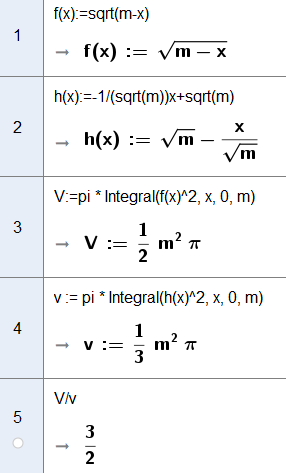
\includegraphics[width=0.7\textwidth]{oppgave12.png}
    \caption{Bevist}
    \label{fig:geogebra}
\end{figure}

\bibliographystyle{alpha}
\bibliography{sample}

\end{document}
